a. The best straight line through the Massachusetts funding/graduation rate data has the equation
$y=81.088+0.412x$, where $s=11.78848$. Construct a $95\%$ confidence interval for $\beta_1$.\\

b. What does this answer imply about the outcome of testing $H_0:\beta_1=0$ versus $H_1:\beta_1\neq0$ at
the $\alpha=0.05$ level of significance?\\

c. Graph the data and superimpose the regression line. How would you summarize these data, and their
implications, to a meeting of the state School Board?\\\\

\begin{solution}\renewcommand{\qedsymbol}{}\ \\
    Well, given the data, we have that
    
    $$\sum_{i=1}^26(x_i-\bar{x})^2=\sum_{i=1}^26x_i^2-n\bar{x}^2=5365.08-26(13.84615)^2=380.4646$$
    
    Now, $t_{\alpha/2}=2.0639$. So, our confidence interval is
    
    $$[0.412-2.0639(\frac{11.78848}{\sqrt{380.4646}}), 0.412+2.0639(\frac{11.78848}{\sqrt{380.4646}})]$$
    $$=[-0.83535, 1.65935]$$

    Since we see that $0\in[-0.83535, 1.65935]$, we fail to reject $H_0$ at the $0.05$ level of
    significance. Given the data, the fact that $0\in[-0.83535, 1.65935]$ at the $0.05$ significance
    level, and the graph below, we can say with $95\%$ confidence that there is a neutral
    correspondance between spending per student and graduation rate. That is, there is significant
    increase or decrease in graduation rates with respect ot an increase in spending per student.

    \begin{center}
        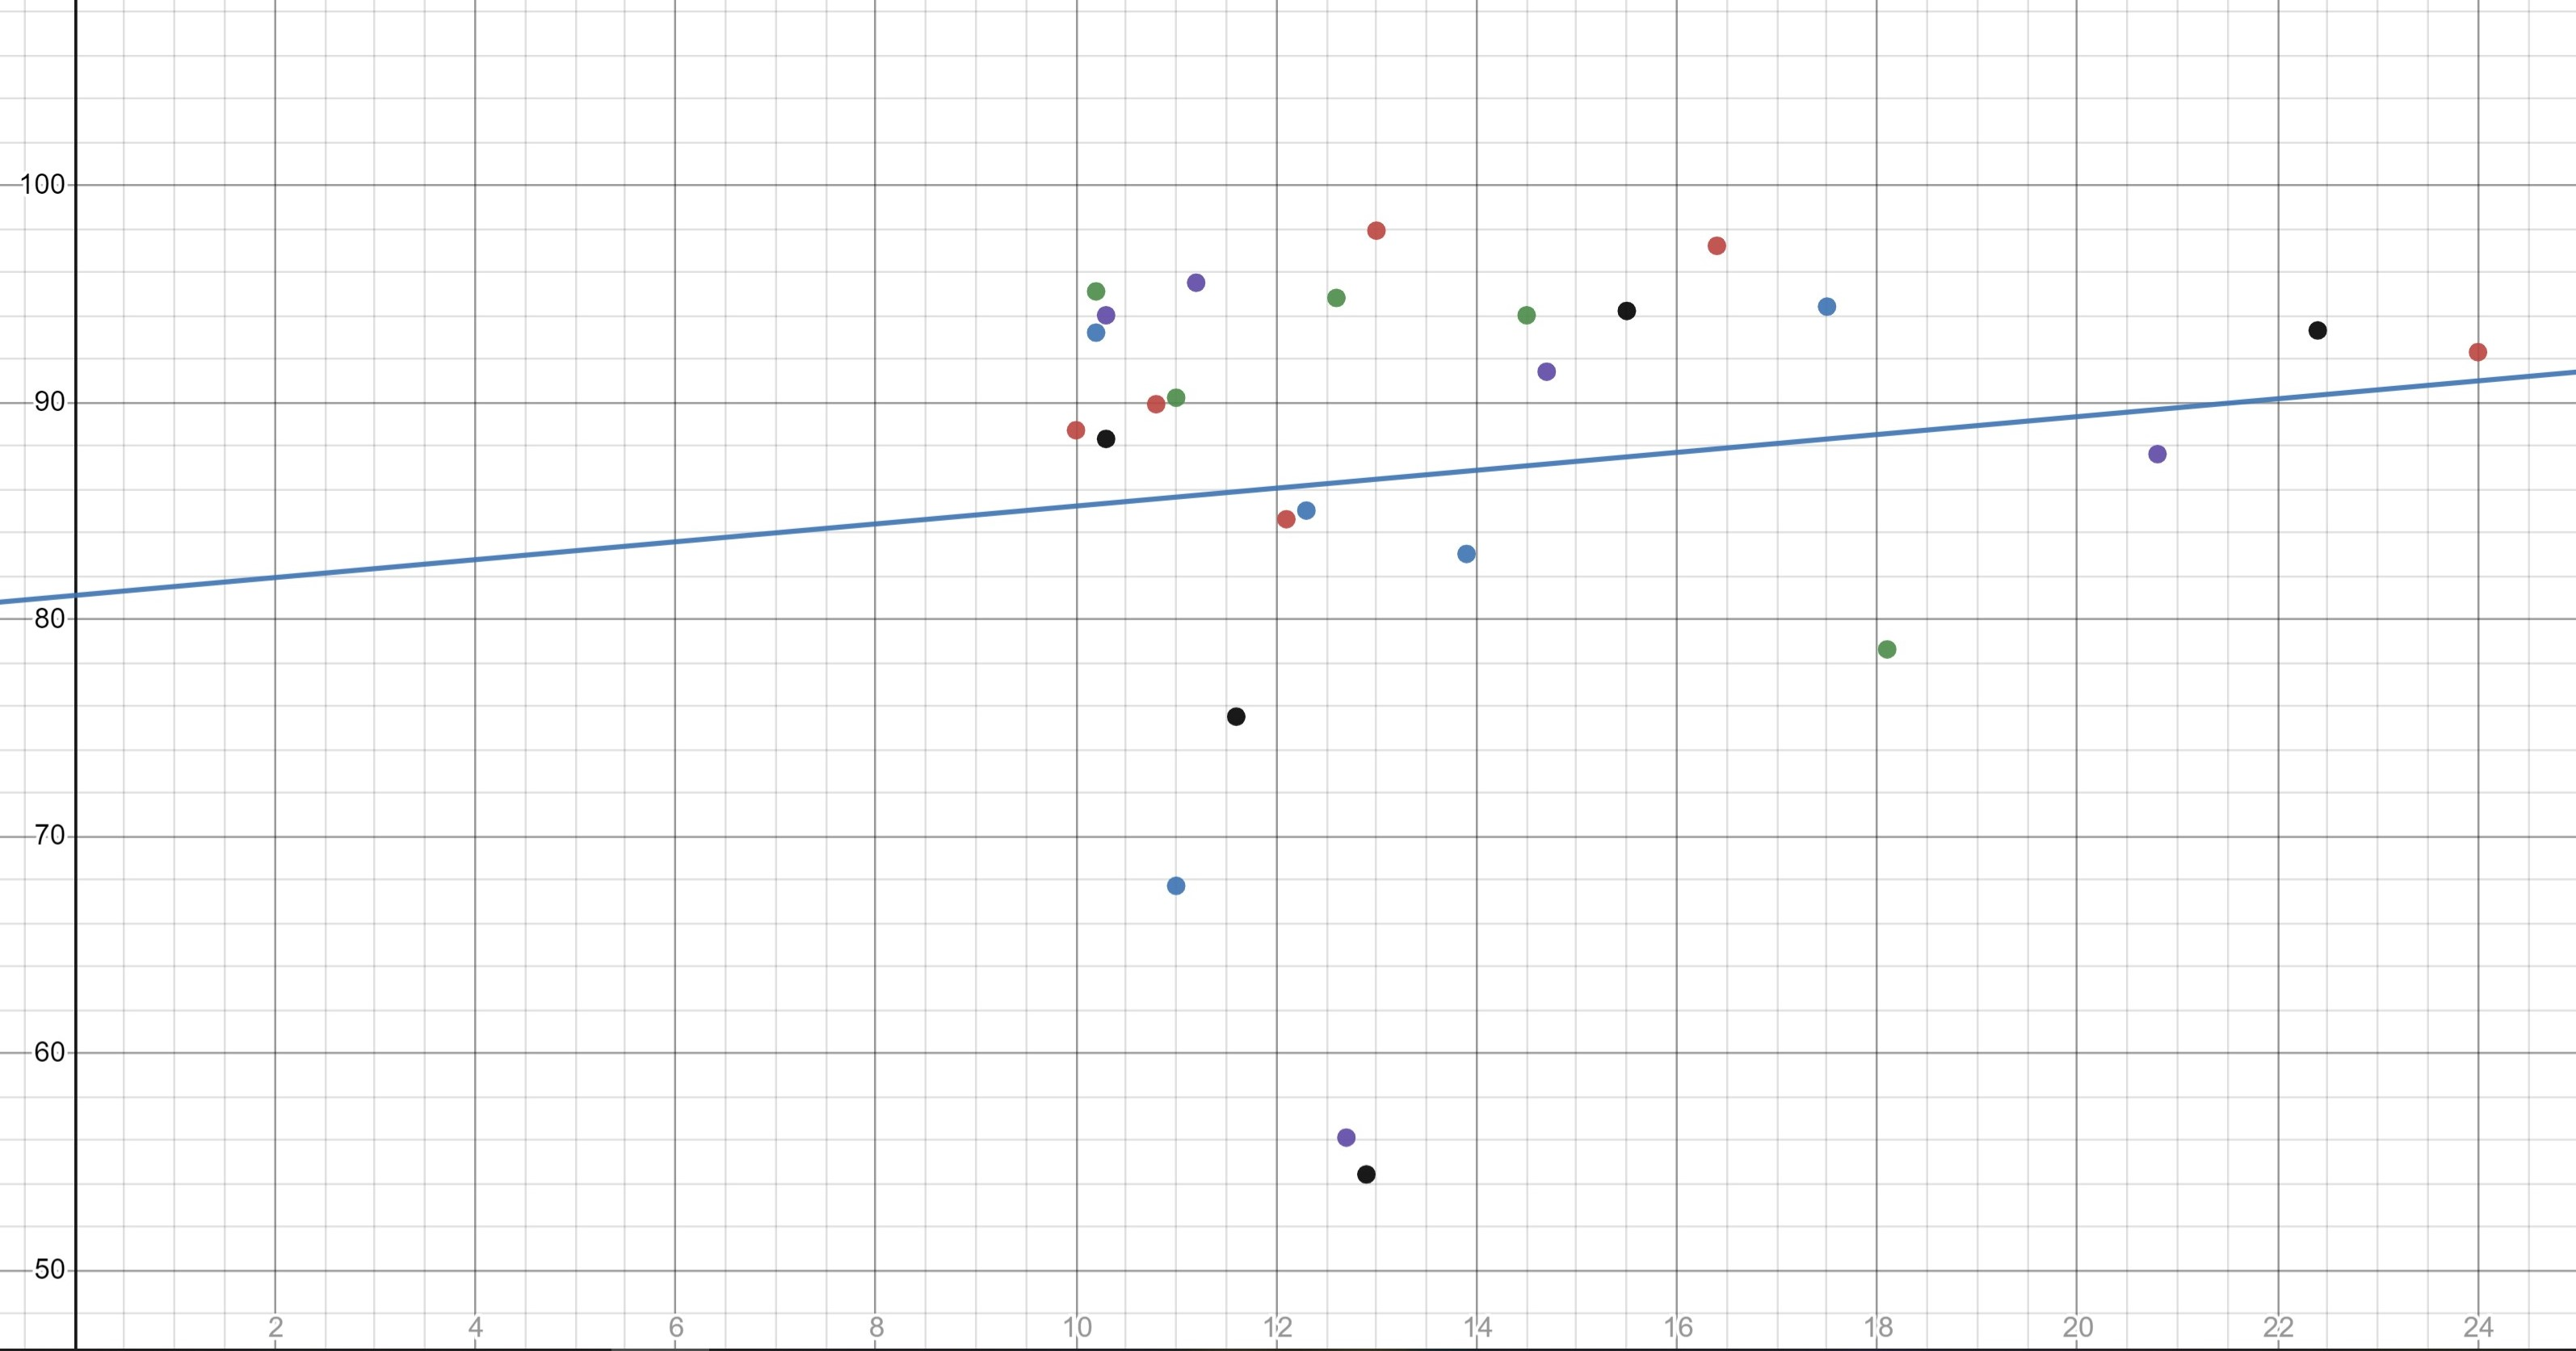
\includegraphics[scale=0.32]{11-3-2.JPG}\\[20pt]
    \end{center}

\end{solution}